\documentclass[output=paper]{LSP/langsci} 
\ChapterDOI{10.5281/zenodo.1291930}
\author{Uwe Reinke\affiliation{Cologne University of Applied Sciences} }
\title{State of the art in Translation Memory Technology} 
\abstract{Commercial Translation Memory systems (\textsc{tm}) have been available on the market for over two decades now. They have become the major language technology to support the translation and localization industries. The following paper will provide an overview of the state of the art in \textsc{tm} technology, explaining the major concepts and looking at recent trends in both commercial systems and research. The paper will start with a short overview of the history of \textsc{tm} systems and a description of their main components and types. It will then discuss the relation between \textsc{tm} and machine translation (\textsc{mt}) as well as ways of integrating the two types of translation technologies. After taking a closer look at data exchange standards relevant to \textsc{tm} environments, the focus of the paper then shifts towards approaches to enhance the retrieval performance of \textsc{tm} systems looking at both non-linguistic and linguistic approaches.}
\maketitle

\begin{document}

%uwe.reinke@fh-koeln.de         

\section{Introduction}\label{sec:reinke:1}

Translation Memory (\textsc{tm}) systems are the most widely used software applications in the localization of digital information, i.e. the translation and cultural adaptation of electronic content for local markets. The idea behind its core element, the actual ``memory'' or translation archive, is to store the originals and their human translations of e-content in a computer system, broken down into manageable units, generally one sentence long. Over time, enormous collections of sentences and their corresponding translations are built up in the systems. \textsc{tm}s allow translators to recycle these translated segments by automatically proposing a relevant translation from the memory as a complete (``exact match'') or partial solution (``fuzzy match'') whenever the same or a similar sentence occurs again in their work. This increases the translator's productivity and helps ensure that the same terminology and expressions are consistently used across translations. Thus, \textsc{tm}s facilitate and speed-up the translation of a rapidly growing amount of specialised texts.

No other technology has changed the general conditions of translation as a professional service as radically as \textsc{tm} systems have done over the past 20 years. This might be due to the fact that \textsc{tm}s mainly support professional translators in their routine work without radically influencing cognitive translation processes in those situations that require the creativity and knowledge of the human translator.

Today most professional translators use \textsc{tm} technology on a regular basis \citet{Massion2005,Lagoudaki2006}. The most well-known commercial systems are \textit{Across, Déjà Vu,} \textit{memoQ,} \textit{MultiTrans,} \textit{\textsc{sdl} Trados,} \textit{Similis,} \textit{Transit} and \textit{Word\-fast}.\footnote{For a brief overview on \textsc{tm} technology see also \citet{Somers2003} and \citet{Reinke2006}. Comprehensive investigations can be found in \citet{Reinke2004}.}

\section{Translation memory systems}\label{sec:reinke:2}
\subsection{History}\label{sec:reinke:2.1}

The basic idea of computer-assisted reuse of human translations can be traced back to the 1960s, when the European Coal and Steel Community (\textsc{ecsc}) developed and used a computer system to retrieve terms and their contexts from stored human translations by identifying those sentences whose lexical items most closely matched the lexical items of a sentence to be translated.

The translation of the sentence (i.e. the sentence stored in the database) is not done by the computer, but by a human translator. However, since the data produced by each query are added to the database, the more the system is in use, the greater is the probability of finding sentences that have the desired term in the proper context \citep[27]{ALPAC1966}.

Yet, modern \textsc{tm} systems differ considerably from the former \textsc{ecsc} application. As the quote below from the \textsc{alpac} report shows, the latter was rather something like a bilingual keyword in context (\textsc{kwic}) retrieval tool that mainly served the purpose of showing source language terms and their target language equivalents in their respective contexts. Retrieving previous translation units for reuse was, if at all, a secondary goal:

\begin{quotation}
The system utilized at \textsc{ceca} is one of automatic dictionary look-up with context included. [\ldots] [T]he translator indicates, by underlining, the words with which he desires help. The entire sentence is then keypunched and fed into a computer. The computer goes through a search routine and prints out the sen\-tence or sentences that most nearly match (in lexical items) the sentences in question. The translator then receives the desired items printed out with their context and in the order in which they occur in the source. \citep[27]{ALPAC1966}
\end{quotation}

A much broader reuse of existing machine-readable human translations with a clear focus on facilitating and accelerating revision processing by identifying unchanged passages was envisaged in a model developed by the translation service of the German Federal Army in the early 1970s \citep{Krollmann1971}. Apart from using several lexical databases this model also envisaged subsystems for storing and analysing text corpora and translation archives stored on magnetic tape:

\begin{quotation}
[\ldots] via descriptors or keywords, large batches of text could automatically be searched for particular passages and then be displayed on video screens as an aid to the trans\-lator; [\ldots] For revised new editions of translations only the changed passages would have to be retyped. Insertion of changes and corrections into the old text would auto\-matically be done by computer [\ldots]. \citep{Krollmann1971}
\end{quotation}

At the end of the 1970s European Comission translator Peter \citet{Arthern1979} proposed even more far reaching computer-assisted support for the translator. His suggestions have to be seen in the context of a discussion led at that time within the European Commission about the use of terminology databases and the feasibility of introducing the \textsc{mt} system \textit{Systran}. While \citegen{Krollmann1971} model only seemed to include the reuse of identical text fragments (today known as ``exact matches''), \citeauthor{Arthern1979} suggests a system that can also retrieve from the reference material similar source language sentences and their translations (today known as ``fuzzy matches''):

\begin{quotation}
This would mean that, simply by entering the final version of a text for printing, as pre\-pared on the screen at the keyboard terminal, and indicating in which lan\-guages to compare the new text, probably sentence by sentence, with all the pre\-viously recorded texts prepared in the organization in that language, and to print out \textit{the nearest available equivalent for each sentence} in all the target languages, on different printers.
\end{quotation}

\begin{quotation}
The result would be a complete text in the original language, plus at least partial translations in as many languages as were required, all grammatically correct as far as they went and all available simultaneously. Depending on how much of the new original was already in store, the subsequent work on the target language texts would range from the insertion of names and dates in standard letters, through light welding at the seams between discrete passages, to the translation of large passages of new text with the aid of a term bank based on the organization's past usage. (\citealt[94f.]{Arthern1979}; my emphasis)
\end{quotation}

While \citeauthor{Arthern1979} did not tackle the issue of ``the nearest available equivalent'' -- or ``similarity'' -- in more detail, he even envisaged the possibility of integrating \textsc{tm} and machine translation (\textsc{mt}):

\begin{quotation}
Since this form of machine-assisted translation would operate in the context of a com\-plete text-processing system, it could very conveniently be supple\-mented by `genuine' machine translation, perhaps to translate the missing areas in texts retrieved from the text memory. \citep[95]{Arthern1979}
\end{quotation}

Yet, it took another decade before the ideas sketched by \citeauthor{Krollmann1971} and \citeauthor{Arthern1979} became part of real applications and market-ready systems. The notion of automatically retrieving ``exact matches'' was first implemented in the early 1980s by \textsc{alps} Inc. (later \textsc{alpnet} Corporation) in a simple component called ``Repetitions Processing'' as part of the company's commercial \textsc{mt} system called \textit{Translation Support System}\textsc{ (\textsc{tss}) } \citep{Seal1992}. The reuse of similar sentences (``fuzzy matching'') was supported by the first commercial \textsc{tm} systems like \textit{\textsc{ibm} Translation Manager}, and \textit{Trados Translator's Workbench~II} that did not appear in the market before the early 1990s.\footnote{\citet{Hutchins1998} and \citet[36--41]{Reinke2004} provide further information on the history of \textsc{tm} systems.}

\subsection{Components}\label{sec:reinke:2.2}

Apart from the ``memory'' or translation archive as its core element, a typical \textsc{tm} system consists of an array of tools and functionalities to assist the human translator. These usually include:

\begin{itemize}
\item 
a \textsc{multilingual editor} for reading source texts and writing translations in all relevant file formats of different word processing programs, \href{http://ecolore.leeds.ac.uk/xml/materials/overview/glossary.xml?lang=en#dtp}{\textsc{dtp} systems}, etc., protecting the layout \href{http://ecolore.leeds.ac.uk/xml/materials/overview/glossary.xml?lang=en#tag}{tags} of these formats against accidentally being deleted or overwritten
\item  
a \textsc{terminology management program} for maintaining termbases to store, retrieve, and update subject-, \href{http://ecolore.leeds.ac.uk/xml/materials/overview/glossary.xml?lang=en#term_entry}{customer-}, and project-specific terminology
\item 
an \textsc{automatic term recognition} \textsc{feature }for automatically looking up in the \href{http://ecolore.leeds.ac.uk/xml/materials/overview/glossary.xml?lang=en#termbase}{termbase} all \href{http://ecolore.leeds.ac.uk/xml/materials/overview/glossary.xml?lang=en#term}{terms} that occur in the source text segment the translator is currently working on
\item 
a \textsc{concordance tool} allowing users to retrieve all instances of a specific search string (single words, word groups, phrases, etc.) from a \href{http://ecolore.leeds.ac.uk/xml/materials/overview/glossary.xml?lang=en#translation_memory}{\textsc{tm}} and view these occurrences in their immediate context
\item 
a \textsc{statistics feature} providing a rough overview of the amount of text that can be reused from a \textsc{tm} for translating a new source document
\item 
an \textsc{alignment tool} to create \textsc{tm} databases from previously translated documents that are only available as separate source and target text files by comparing a source text and its translation, matching the corresponding \href{http://ecolore.leeds.ac.uk/xml/materials/overview/glossary.xml?lang=en#segment}{segments}, and binding them together as \href{http://ecolore.leeds.ac.uk/xml/materials/overview/glossary.xml?lang=en#translation_unit}{units} in a \textsc{tm}.
\end{itemize}

In addition, a few \textsc{tm} systems offer terminology extraction as an optional or an integrated feature to assist in populating termbases and setting up the terminology for an e-content localization project by extracting mono- or bilingual lists of potential terms from a selection of electronic (source and/or target) texts. Today, many \textsc{tm} suites also include support for machine translation, either by offering interfaces with \textsc{mt} systems or even by integrating their own \textsc{mt} component. Finally, some kind of project management (\textsc{pm}) support is built into most \textsc{tm} systems. These \textsc{pm} features may support:

\begin{itemize}
\item 
file handling and management (specification of all source language files, project-relevant termbases and \textsc{tm} databases, assistance in defining folder structures)
\item 
management of client and translator data (addresses, contact persons, translators' skills, equipment, availability, etc. )
\item 
workflow management (deadlines, project progress, etc.).
\end{itemize}

\figref{fig:reinke:1} provides an overview of how the major components of a standard \textsc{tm} environment interact, while \figref{fig:reinke:2} gives an example for a typical user interface of a commercial \textsc{tm} system.

\begin{figure}[h]
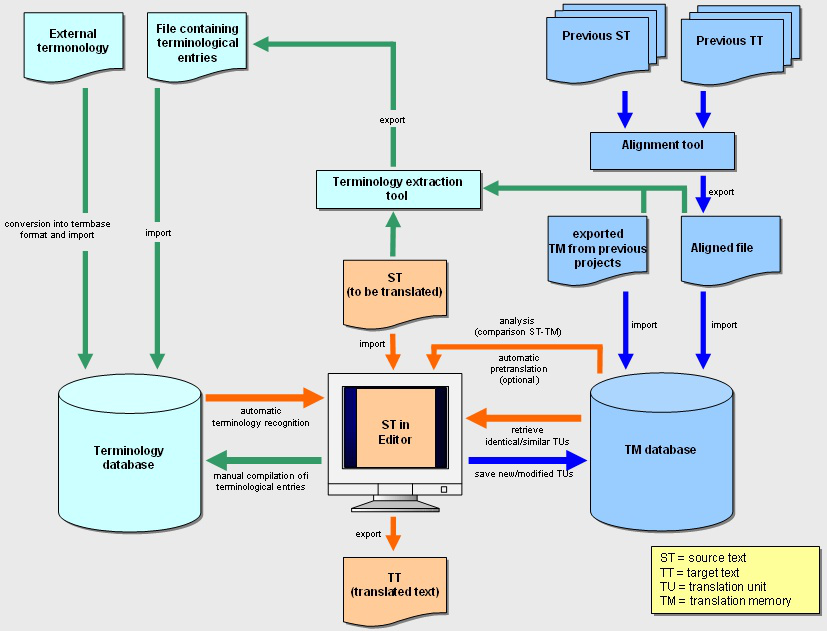
\includegraphics[width=\textwidth]{figures/ReinkeF1.png}
\caption{Components and processes in a translation memory (\textsc{tm}) system (excluding project management and machine translation functionalities)}
\label{fig:reinke:1}
\end{figure} 

\begin{figure}[h]
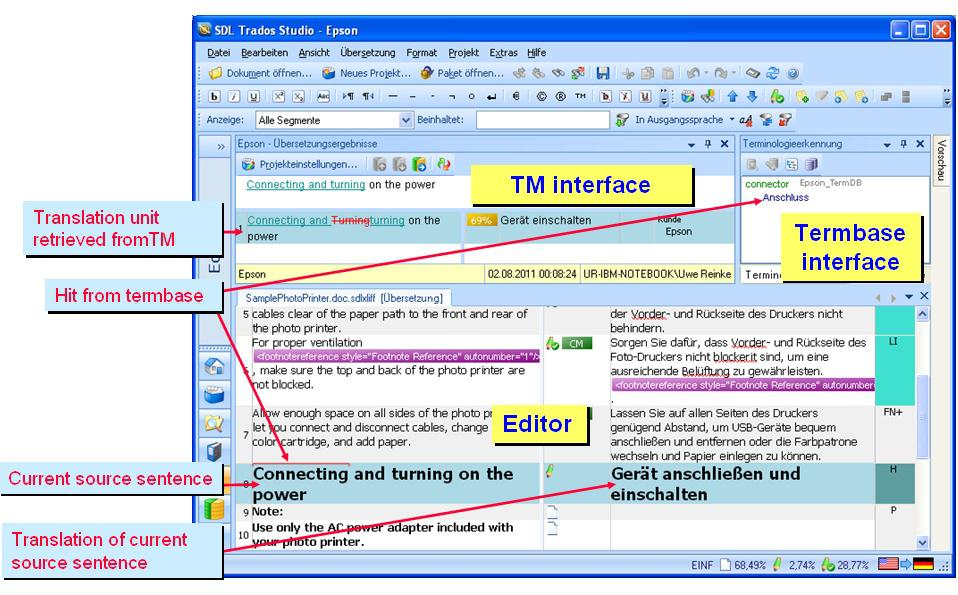
\includegraphics[width=\textwidth]{figures/ReinkeF2.png}
\caption{User interface of \textsc{sdl} Trados Studio}
\label{fig:reinke:2}
\end{figure}

Although professional translators often stress the need to constantly adjust to rapid technological changes in the field (some complaining about this constant pressure, others rather regarding it as a professional necessity and a challenge), it must be said that all in all the core functionalities of commercial \textsc{tm} systems have remained very much the same since the first -- mostly still \textsc{ms-dos}-based -- applications became available at the beginning of the 1990s. Even the first versions contained a translation memory, a terminology management system and a (multilingual) editor, providing features like exact and fuzzy matching, pretranslation\footnote{Pre-translation refers to the batch process ``of comparing a complete source text to a Translation Memory database and automatically inserting the translations of all exact matches found in the database. The result is a hybrid text containing pretranslated and untranslated segments.'' \citep{eCoLoRe2012}}, concordance lookup, terminology recognition, etc. (\figref{fig:reinke:3}). Of course, the matching algorithms -- although still being based on simple character matching procedures -- have been altered and modified to a considerable extent, and many additional features and functionalities have been added, so that a growing number of scholars, professionals and application providers now prefer to call \textsc{tm} systems ``translation environments'' or ``translation environment tools (TEnT)'' \citep[8]{CERTT2012}.

\begin{figure}[h]
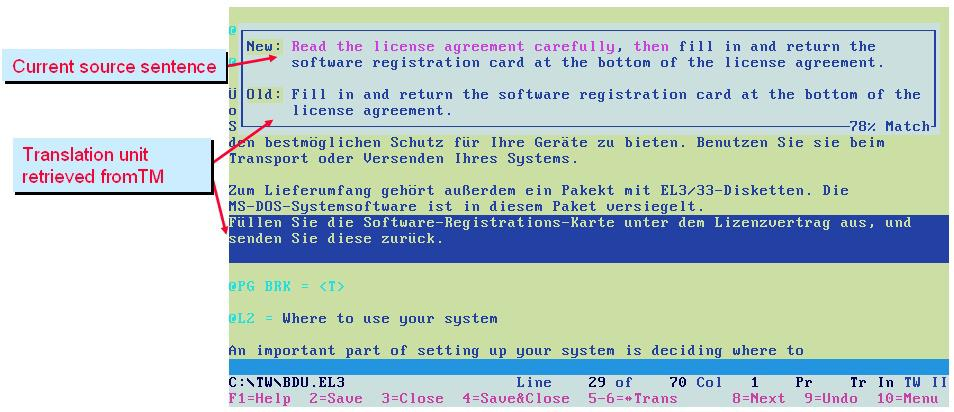
\includegraphics[width=\textwidth]{figures/ReinkeF3.png}
% \end{figure}
% \begin{figure}
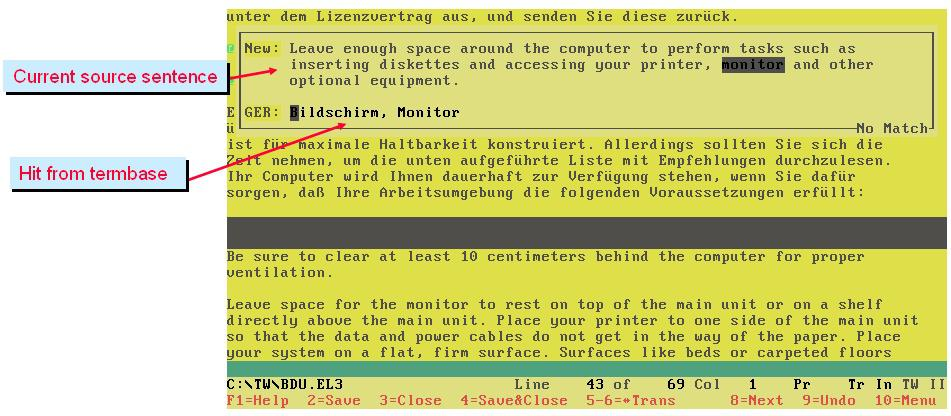
\includegraphics[width=\textwidth]{figures/ReinkeF3a.png}
\caption{Fuzzy matching and terminology recognition in TRADOS Translator's Workbench II}
\label{fig:reinke:3}
% \label{fig:reinke:3a}
\end{figure}

What has changed dramatically indeed during the last two decades is the translation workflow, i.e. the way the translation processes are organized and the way the parties involved in these processes interact and collaborate. The introduction of client/server solutions after the turn of the millennium enabled new ways of real-time collaboration among distributed teams but led to even more controversial discussions about intellectual property rights on \textsc{tm} data collections and liability issues. The near future will reveal to which extent new buzzword technologies and forms of collaboration like ``cloud computing'' and ``crowd sourcing'' will actually affect translation workflows and work situations.

\subsection{Types of TM systems}\label{sec:reinke:2.3}

In most systems available on the market the \textsc{tm} is a database. Each record in a \textsc{tm} database contains a translation unit (\textsc{tu}) consisting of a pair of source and target text segments.\footnote{In most \textsc{tm}s, translation units consist of source language sentences and their target language equivalents. Apart from 1:1 equivalences, where a sentence from the source text is transferred into one sentence in the target text, this can also include 1:n and n:1 relations, depending on the decisions taken by the individual translator. Moreover, smaller \textsc{tu}s having the size of clauses or phrases, larger units based on paragraphs, or nested units starting at paragraph level and then assigning further relations at sentence level may also occur.} In addition to the \textsc{tu}, there may be further information on the creation and modification dates, the person who created or modified the entry, the project(s) or customer(s) the \textsc{tu} is used for, etc.

A major feature of a typical \textsc{tm} database is the fact that it grows incrementally. The database is `dynamic' because new \textsc{tu}s -- regardless of whether they are created from scratch or by adjusting the translation of a similar \textsc{tu} retrieved from the \textsc{tm} -- are added during the translation process. \largerpage

Basically, there are three ways of feeding a \textsc{tm}:

\begin{itemize}
\item 
While translating: When translating a text using a \textsc{tm} database each segment from the source text will be automatically stored in the database along with its translation.
\item 
By importing another \textsc{tm} database: This can either be a \textsc{tm} created with the same \textsc{tm} system or a \textsc{tm} available in the Translation Memory eXchange format (\textsc{tmx}), which is supported by all commercial systems.
\item 
By aligning existing translations and their original texts: With the help of an alignment tool it is possible to create \textsc{tm} databases from the source and target text files of previous translation projects.
\end{itemize}

Some \textsc{tm} systems do not make use of the database approach but store entire source and target text pairs in their proprietary formats as reference material for future reuse in related translation projects. While \textsc{tm} databases constitute an amalgamation of translation units that isolates each segment from its context, the reference text approach makes it easier to take context into account during the matching process. On the other hand, this approach is rather static, i.e. it is not possible to immediately reuse \textsc{tu}s that have just been created. Therefore, systems based on the reference text approach also create a so called temporary ``fuzzy index'', which is a kind of temporary database providing access to recently created \textsc{tu}s as well as fuzzy-match functionality. In turn, \textsc{tm} systems following the database approach have tried to overcome the complete decontextualisation of their \textsc{tu}s by adding so-called ``context matches'' or ``perfect matches'', where an exact match is preceeded and/or followed by another exact match, i.e. the segment to be translated and the match retrieved from the \textsc{tm} have the same textual environment. This is achieved by simply storing in the \textsc{tm} database the relevant context segments together with the actual \textsc{tu}s and sometimes by additionaly taking into account information obtained from style sheets, document templates or structural document markup \citep{Chama2010}. Some database-oriented \textsc{tm} systems have also included the reference text approach as an additional option to retrieve translaslation units for reuse by allowing to specify bilingual files from previous translation projects and combining them with \textsc{tm} databases. In general, it seems that the developers of commercial \textsc{tm} systems more and more try to combine the advantages of both the database-oriented and the reference text-oriented approaches.

Another major issue in \textsc{tm} technology is the retrieval of fragments below sentence level. Most commercial \textsc{tm} systems now offer some kind of subsegment matching. The simplest form of subsegment matching is to look for complete \textsc{tm} database and termbase units that are part of the current souce language segment and automatically insert their target language sections, thus usually creating suggestions that form a mix of source and target language fragments and require further adaptation (``fragment assembly''). A more complex way of finding subsegments is to retrieve longest common substrings (\textsc{lsc}s) from \textsc{tm} database units (\figref{fig:reinke:4}). Finally, a third -- and probably the most productive -- way of subsegment matching that can be found in commercial \textsc{tm} systems is to automatically suggest target language fragments while typing a translation (auto-completion; \figref{fig:reinke:5}). These fragments are retrieved from bilingual lexicons that were statistically generated from \textsc{tm} databases \citep{Chama2010}.

\begin{figure}
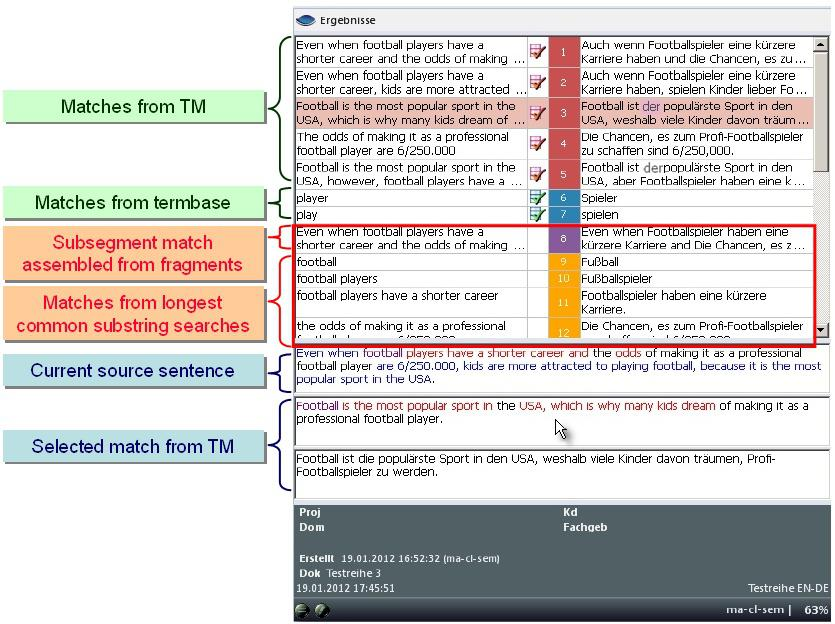
\includegraphics[width=\textwidth]{figures/ReinkeF4.png}
\caption{Subsegment matching in Kilgray MemoQ}
\label{fig:reinke:4}
\end{figure}

\begin{figure}
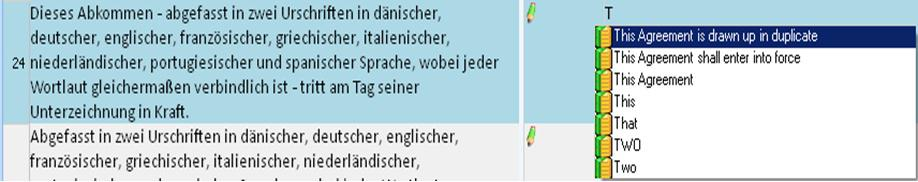
\includegraphics[width=\textwidth]{figures/ReinkeF5.png}
\caption{Subsegment matching in \textsc{sdl} Trados Studio }
\label{fig:reinke:5}
\end{figure}

\subsection{Translation memory and machine translation}\label{sec:reinke:2.4}
\subsubsection{Distinction between TM and MT}\label{2.4.1}

\textsc{tm} technology is not to be confused with machine translation. Whereas \textsc{mt} translates without human intervention, \textsc{tm} systems provide features and tools to store and retrieve segments translated by a human translator. Despite this essential distinction between \textsc{tm} and \textsc{mt}, \textsc{tm} technology shares certain commonalities with both example-based machine translation (\textsc{ebmt}), an approach first suggested in Japan in the early 1980s \citep{Nagao1984}, and statistical machine translation (\textsc{smt}), an approach developped at \textsc{ibm} in the late 1980s \citep{BrownEtAl1988} that did not have its breakthrough before the turn of the millenium and is considered the state-of-the art paradigm in \textsc{mt} today \citep[17f]{Koehn2010}. Both \textsc{tm} and \textsc{ebmt}/\textsc{smt} try to retrieve ``best matches'' for the sentences of the text to be translated from a bilingual text archive or database containing sentence-level alignments of existing translations and their original texts.\footnote{Both \textsc{ebmt} and \textsc{smt} are corpus-based approaches, so that the term corpus-based \textsc{mt} (\textsc{cbmt}) is used as an umbrella for both as opposed to rule-based \textsc{mt} (\textsc{rbmt}) \citep[xviii]{Carl2003}. The major difference between \textsc{ebmt} and \textsc{smt} is that \textsc{smt} considers translation as a ``statistical optimization problem'' \citep[17]{Koehn2010} and is based on probability calculations over large bilingual corpora, while \textsc{ebmt} tries to find analogies between an input sentence and examples from a bilingual corpus applying more ``traditional'' linguistic means like (morpho-)syntactic analysis and thesauri. For an extensive overview on \textsc{ebmt} see \citet{Carl2003} and \citet{Somers2001}. A comprehensive introduction to \textsc{smt} can be found in \citet{Koehn2010}.} Yet, there are fundamental differences between the purposes of \textsc{ebmt}/\textsc{smt} and \textsc{tm} systems. A \textsc{tm} is mainly an information retrieval application that leaves decisions about whether and how to reuse and adjust the retrieved results -- and thus the actual translation task -- to the human translator. \textsc{ebmt} and \textsc{smt} produce translations by automatically selecting suitable fragments from the source language side of the retrieved \textsc{tu}s and building the translation from the corresponding elements of the target language side. Due to the complexity of this recombination task, not every \textsc{tu} contained in a translation archive is equally suited for reuse in \textsc{tm} systems and \textsc{ebmt} or \textsc{smt} environments. \largerpage %widow

\subsubsection{Integration of TM and MT}\label{sec:reinke:2.4.2}

For good reason \textsc{mt} has so far been used very little in high quality e-content localization. \textsc{mt} is only suited for a very limited range of text types, and source texts have to be carefully tailored to the capabilities and restrictions of an \textsc{mt} system to minimize the amount of time and effort needed for post-editing.

Nevertheless, \textsc{tm} suites increasingly offer support for \textsc{mt}. Basically, there are two possible ways of combining \textsc{mt} and \textsc{tm}:

\begin{enumerate}
\item 
Batch processing (usually during data preparation):
In a batch scenario, all segments of the source text that do not produce an exact or high percentage ``fuzzy match'' when being compared with the \textsc{tm} database may be exported for processing by \textsc{mt}. After the unknown segments have been translated by the \textsc{mt} application, the new translation units can be merged into the \textsc{tm} database. When the translator works on the text, the units generated by the \textsc{mt} system will be presented as candidate translations, possibly with a predefined matching penalty.
\item
Interactive processing (during the translation stage proper):
In an interactive scenario, translators can invoke the \textsc{mt} system each time there is no match with the \textsc{tm} database. If the result from the \textsc{mt} system proves helpful, it can be edited as necessary. The resulting translation unit will then be stored in the \textsc{tm} database for future reuse.
\end{enumerate}

Commercial \textsc{tm} systems like \textit{Across} or \textit{\textsc{sdl} Trados Studio} offer interfaces to both \textsc{rbmt} and \textsc{smt} systems. Large \textsc{MT} companies like \textit{Sybase} report productivity gains by combining \textsc{smt} and \textsc{tm}, provided that the \textsc{mt} system has been trained with a large-enough company-specific bilingual corpus (cf. Bier 2012). Like other large companies \textit{Sybase} has carried out experiments using the freely available \textsc{smt} system \textit{Moses} \citep{KoehnEtAl2007} interactively together with a \textsc{tm} system. \citet{Bier2012} mentions faster turnaround (delivery time decreased by an average of 50\%), 20--30\% cost reductions for updates, stable translation quality (no visible impact on style with full post-editing, fewer content errors, slight increase in minor linguistic errors) and a rise in productivity between 5 and 70\% (depending on the kind of source texts, the terminology used and the performance of individual translators).\footnote{For a comparison of \textsc{tm} and \textsc{smt} output see also \citet{OffersgaardEtAl2008}.
\citeauthor{OffersgaardEtAl2008} report high productivity gains of more than 65\% for certain domains and for situations in which the \textsc{tm} database does not produce matches for two thirds or more of the sentences to be translated. \citet{Guerberof2009} also reports higher processing speed for post-editing \textsc{smt} output compared with \textsc{tm} matches, but also points to the fact that deviation between individual subjects is very high.}

\subsection{Data exchange standards for TM systems}\label{sec:reinke:2.5}
\subsubsection{Overview}\label{sec:reinke:2.5.1}
 
A versatile \textsc{tm} system must be able to handle the full range of proprietary and standard file formats in which e-content can be produced and exchanged. One of the major metastandards that play a central role in technical documentation is the eXtensible Markup Language (\textsc{xml}) \citep{W3C2008}. \textsc{xml} provides a framework for the creation of markup languages for all kinds of individual document types, and there is a growing number of \textsc{xml}-based standards and formats to support various aspects of the documentation and localization process. While standards like DocBook \citep{OASIS2006}, \textsc{dita} \citep{OASIS2007}, and \textsc{xliff} \citep{OASIS2008} are related to the creation and exchange of localizable content, \textsc{tmx} \citep{LISA2005}, \textsc{srx} \citep{LISA2008} and \textsc{tbx} \citep{ISO2008} serve the purpose of facilitating the exchange of reference material (\textsc{tm} databases and termbases). 
 
Current efforts like Linport (Language Interoperability Portfolio, \citealt{Linport2012}) and \textsc{tipp} (Translation Interoperability Protocol Package, \citealt{InteroperabilityNow!2012}) focus on the development of a standard for the exchange of complete translation projects between different translation environments.

\subsubsection{Supporting standards for the exchange of localizable e-content}\label{sec:reinke:2.5.2}
 
For public \textsc{xml}-based standards like DocBook, \textsc{dita} und \textsc{xliff}, \textsc{tm} systems should include import routines that provide an automatic distinction between so-called ``external'' \textsc{xml} markup elements, that need not be modified during the translation process, and ``internal'' elements, which the translator may need to move, add or delete. Translatable and non-translatable attribute values should be distinguished automatically as well.
 
For proprietary \textsc{xml}-based formats, \textsc{tm} systems should provide a feature to create import routines from a combination of various sources, i.e. \textsc{xml} document type definitions (\textsc{dtd}s), \textsc{xml} schema definition files (\textsc{xsd}s) and localizable \textsc{xml} content files, keeping the effort for manually correcting translation-related settings for the indiviudal \textsc{xml} elements and attributes as small as possible.
 
Content in formats like \textsc{xliff}, which mainly serve the purpose of exchanging bilingual files during the localization process, must be diplayed correctly in the \textsc{tm} system's multilingual editor, i.e. for editors using separate windows or table columns for source and target languages, the {\textless}source{\textgreater} and {\textless}target{\textgreater} elements of an \textsc{xliff} file must be placed into the correct windows or columns (\figref{fig:reinke:6}). Moreover, metadata like translation comments and information on the processing status of translation units should be adequately imported, displayed and exported without any loss of information (\figref{fig:reinke:7}).
 
Finally, it must be taken into account that \textsc{xliff} is a kind of hybrid format, because apart from localizable content \textsc{xliff} files can also contain bilingual reference material from previous versions or related documents. \textsc{tm} systems must be able to recognize this reference material in an \textsc{xliff} file and store it in a \textsc{tm} database together with relevant metadata also contained in the \textsc{xliff} file, like information on match values, authors, systems used to create the material, etc. (\figref{fig:reinke:8}).

\begin{figure}
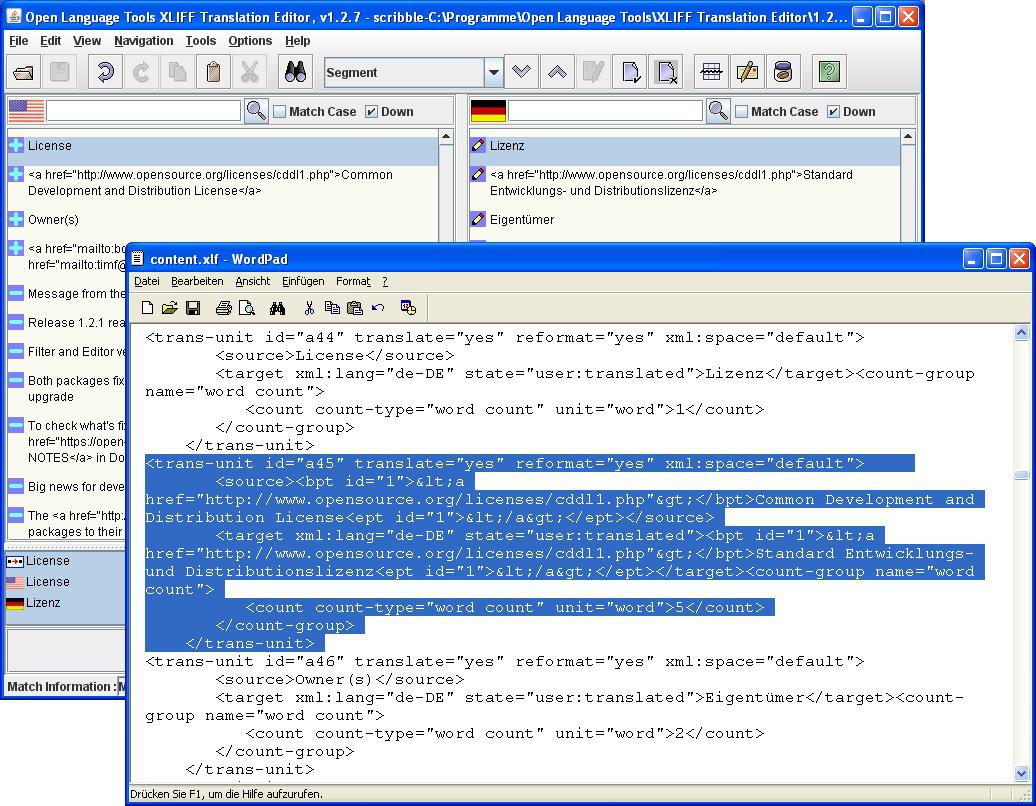
\includegraphics[width=\textwidth]{figures/ReinkeF6.png}
\caption{Fragment from an \textsc{xliff} file in a text editor and in an \textsc{xliff} translation editor}
\label{fig:reinke:6}
\end{figure}

\begin{figure}
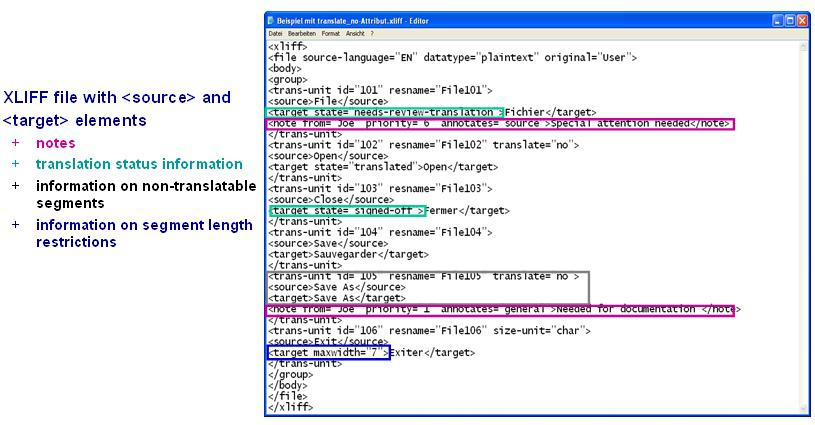
\includegraphics[width=\textwidth]{figures/ReinkeF7.png}
\caption{Complex \textsc{xliff} file containing various metadata}
\label{fig:reinke:7}
\end{figure}

\begin{figure}
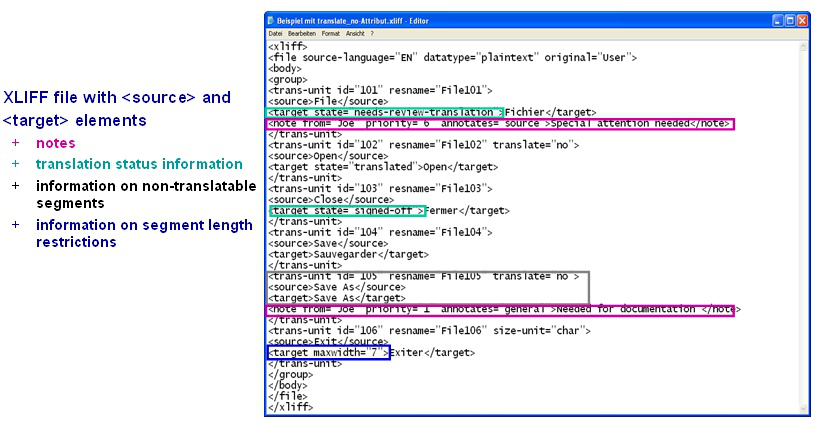
\includegraphics[width=\textwidth]{figures/ReinkeF8.png}
\caption{\textsc{xliff} file containing various reference material}
\label{fig:reinke:8}
\end{figure}

\subsubsection{Supporting standards for the exchange of reference material}\label{sec:reinke:2.5.3}

The exchange of \textsc{tm} database elements mainly causes problems with respect to the maintenance of layout information and dynamic fields (i.e. placeholders for embedded objects and automatically adjustable content like cross-references and other variables) contained in \textsc{tu}s and the exchange of information on rules used for the segmentation of text into \textsc{tu}s.

To keep the loss of layout-related information and placeholders for embedded objects and dynamic fields contained in \textsc{tu}s as minimal as possible when exchanging \textsc{tm}s between different applications most \textsc{tm} systems support \textsc{tmx} Level~2. The \textsc{tmx} standard has been available since 1998. It has been developed by the Localization Industry Standards Association (\textsc{lisa}), which was an interest group of major information technology companies and localization service providers. After \textsc{lisa} became insolvent in 2011. \textsc{tmx} is now being maintained by the Localization Industry Standards (\textsc{lis}) Industry Specification Group (\textsc{isg}) of the European Telecommunications Standards Institute (\textsc{etsi}) \citep{GALA2012} and the standard is freely available from the website of the Globalization and Localization Association (\textsc{gala}).\footnote{\textsc{gala} is a non-profit organization of localization and translation service providers, language technology developers and other companies involved in language services or technology. The former \textsc{lisa} standards can be found at \url{http://www.gala-global.org/lisa-oscar-standards}.}
 
Breaking up text into smaller \textsc{tu}s requires segmentation rules that may differ between languages as well as text types and file formats. Examples include individual punctuation characters like the quotation mark in Spanish or the different treatment of colons, semi-colons and other characters depending on language and text type. In order to overcome a loss in reusability of \textsc{tu}s due to different segmentation rules applied in different \textsc{tm}s the Segmentation Rules eXchange (\textsc{srx}) standard was introduced in 2004. The segmentation rules contained in an \textsc{srx} file (\figref{fig:reinke:9}) must be applied when exporting and importing \textsc{tm}s as well as during the actual translation process when the current source text has to be split up into \textsc{tu}s.

Like \textsc{tmx}, \textsc{srx} was developed by \textsc{lisa} and is now being maintained by \textsc{etsi}. It can also be downloaded from the \textsc{gala} website.

\begin{figure}
% 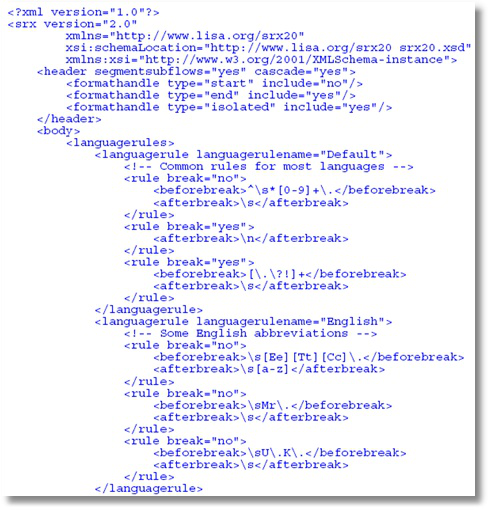
\includegraphics[width=\textwidth]{figures/ReinkeF9.png}
\begin{lstlisting}
<?xm1 version="1.0"?>
<srx version="2.0"
    xmlns="http://www.lisa.org/srx20"
    xsi:schemaLocation="http://www.lisa.org/srx20 srx20.xsd"
    xnlns:xsi="http://www.v3.org/2001/XMLSchena-instance">
  <header segmentsubflows="yes" cascade="yes">
    <formathandle type="start" include="no"/>
    <formathandle type="end" include="yes"/>
    <formathand1e type="isolated" include="yes"/>
  </header>
  <body>
    <languagerules>
      <languagerule languagerulename="Default">
      <!-- Common rules for most languages -->
      <rule break="no">
	  <beforebreak>^\s*[0-9]+\.</beforebreak>
	  <afterbreak>\s</afterbreak>
      </rule>
      <rule break="yes">
	  <afterbreak>\n<afterbreak>
      </rule>
      <rule break="yes">
	  <beforebreak>[\.\?!]+</beforebreak>
	  <afterbreak>\s</afterbreak>
      </rule>
    </languagerule>
    <languagerule languagerulename="English">
      <!-- Some English abbreviations -->
      <rule break-“no'>
	<beforebreak>\s[Ee][Tt][Cc]\.</beforebreak>
	<atterbreak>\s[a-z]</afterbreak>
     </rule>
     <rule break="no">
	  <beforebreak>\sMr\.</beforebreak>
	  <afterbreak>\s</afterbreak>
      </ru1e>
      <rule break="no">
	  <beforebreak>\sU\.K\.</beforebreak>
	  <afterbreak>\s</afterbreak>
      </ru1e>
     </languagerule>
\end{lstlisting}

\caption{Section from an \textsc{srx} file}
\label{fig:reinke:9}
\end{figure}

Exchanging data between the terminology management components of various \textsc{tm} systems can be much more challenging than sharing \textsc{tm}s among various applications. This is due to the fact that the structure and complexity of termbases may differ severely from system to system and -- in the case of user-definable entry structures -- even among termbases created with the same application. It has taken a long time since the efforts to define a universal exchange format for terminological data have lead to the Termbase eXchange Standard (\textsc{tbx}). Although \textsc{tbx} has become an \textsc{iso} standard in 2008 (cf. \citealt{ISO2008}) the format is still not properly supported by all \textsc{tm} systems.

\subsection{Advantages and limitations of TM systems}\label{sec:reinke:2.6}
 
The advantages of using \textsc{tm} systems are fairly obvious: they increase the translator's productivity and enhance translation quality by ensuring that terminology and expressions are used consistently within and across translations. Users in industry and international organizations usually claim a 25\% to 60\% rise in productivity \citep[113f.]{Reinke2004}. However, at least in some industries productivity gains seem to come to an end after a certain time. Thus, at Sybase ``[t]raditional \textsc{tm} technology [is] almost fully exploited'' with ``ca. 80\% of costs spent on `new' words'' and ``only 20\% spent on recycling'' \citep{Bier2012}. Bier also states that there are ``[n]o more improvements in turnaround times'' as the average productivity of translators has remained at a maximum level of 2.400 words per day for years.
 

\begin{figure}
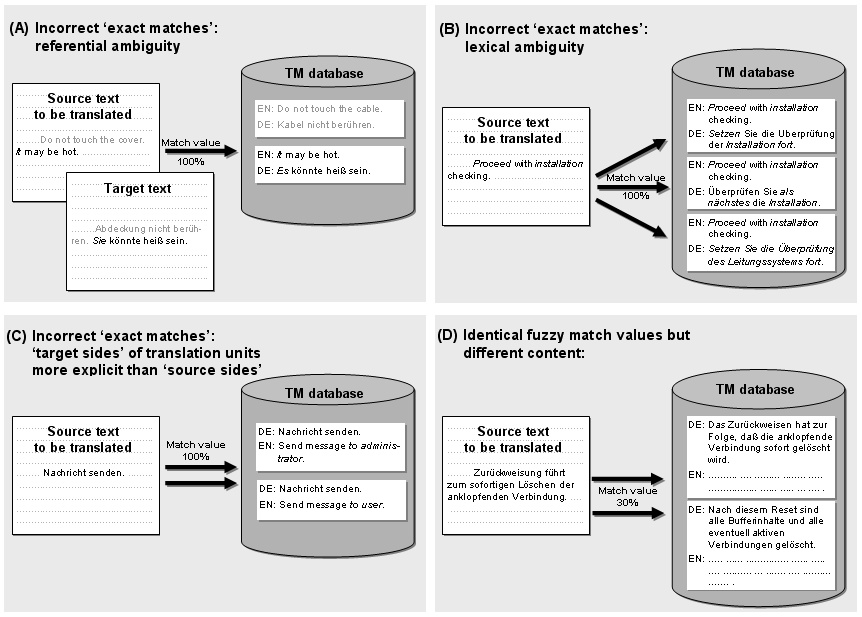
\includegraphics[width=\textwidth]{figures/ReinkeF10.png}
\caption{Examples in English (\textsc{en}) and German (\textsc{de}), demonstrating shortcomings of fuzzy match algorithms \citep[64]{Reinke2006}}
\label{fig:reinke:10}
\end{figure}
 
Furthermore, it must be stated that the use of \textsc{tm} systems may also have negative effects on translation quality. One of the major disadvantages of \textsc{tm} systems is that they usually operate at sentence level. Thus, there is a serious danger that the translator will focus too much on isolated sentences, possibly disregarding the contexts they are embedded in \citep[136f.]{Reinke2004}.
 
Examples (A) and (B) in \figref{fig:reinke:10} examplify this problem with respect to referential and lexical ambiguity. In example (A) the pronoun \textit{it} is an anaphoric reference to the noun phrase \textit{the cover} in the previous sentence. As the German translation \textit{die Abdeckung} is female, the pronoun should be female as well (i.e. \textit{sie}). In the same English sentence in the \textsc{tm} the pronoun \textit{it} refers to a different noun phrase with a German translation using a neuter noun like \textit{das Kabel,} so that \textit{it} has to become \textit{es}. Thus, an exact match for \textit{It can be hot} yields a translation that does not fit the current context. In example (B) terms like \textit{installation }or general language words like \textit{proceed} are lexically ambiguous. \textit{Installation} could, for instance, refer the installation of a piece of software or to a piping system, while \textit{to proceed with s.th.} might mean \textit{to continue a process that has been interrupted} or \textit{to go on with the next step of a process}. These different meanings require different translations in German. Therefore, an exact match from the \textsc{tm} might produce an incorrect translation.
 
The matching algorithms of \textsc{tm} systems are based on very simple formal criteria like the similarity of character strings. Thus, the human translator's notion of the degree of similarity between a segment to be translated and a segment retrieved from the database may differ considerably from the degree of similarity calculated by the \textsc{tm} system. This may lead to situations where ``exact matches'' yield wrong translations (examples A to C in \figref{fig:reinke:10}) or one translation of a ``fuzzy match'' requires little or no adjustment, while another ``fuzzy match'' with the same similarity value is not useful at all, e.g., because the content belongs to a different (sub-)domain (example D in \figref{fig:reinke:10}).
 
Despite these drawbacks, it should be noted that \textsc{tm} systems generally integrate into the translation workflow comparatively smoothly. As opposed to \textsc{mt}, they leave human translators in control of the actual translation process, while relieving them from routine work and maintaining translation as a creative act whenever the linguistic resourcefulness of a human being is required.
 
\section{Approaches to enhance the information retrieval performance of TM systems}\label{sec:3}
\subsection{Approaches not applying ``linguistic knowledge''}\label{sec:reinke:3.1}
 
Although commercial \textsc{tm} systems have been available for over two decades, their retrieval performance has not improved considerably in terms of quality and quantity. Of course, the matching algorithms have been altered and modified over time, but they still rely on simple character- or token-based matching procedures without taking into account linguistic aspects like morphosyntactic, syntactic or semantic features that may determine the ``similarity'' of translation units.\footnote{For a brief overview on similarity measures relevant to \textsc{tm} systems see \citet[61--68]{Trujillo1999}, \citet[193--198]{Reinke2004}, \citealt{Sikes2007}.} Even rather straightforward approaches that do not rely on ``linguistic knowledge'' but could, for instance, easily improve the retrieval performance for \textsc{tu}s containing so-called placeable and localizable elements\footnote{Placeable elements like tags, inline graphics and dynamic fields usually do not contain translatable text. They can often be copied (``placed'') into the target text without any need for further modifications. Tags are markup elements in \textsc{html} and \textsc{xml} files; inline graphics and dynamic fields typically occur in \textsc{dtp} formats and Microsoft Word files. Localizable elements like numbers, dates, \textsc{url}s or e-mail addresses, in turn, consist of plain text following a certain pattern, so that they can be identified without any ``linguistic knowledge''. The localization of these elements follows given rules and often does not influence the remaining parts of a \textsc{tu}.} are not yet a matter of course in commercial \textsc{tm} systems.
 
\citet{Azzano2011} presents a detailed analysis of the question at what extent the occurrence of placeable and localizable elements influence the retrieval performance of commercial \textsc{tm} systems. He found that placeable elements sometimes lead to comparatively low fuzzy match values because some systems treat them like standard text when comparing the lengths of source language segments (SegSL) to be translated and source language segments from a \textsc{tm} (SegSL\textsubscript{TM}). Instead, it would be more reasonable to use a fixed penalty when SegSL and SegSL\textsubscript{TM} only differ with respect to the placeable elements they contain while the remaining standard text is identical.
 
\citet{Azzano2011} also reports that some systems yield exact matches when SegSL and SegSL\textsubscript{TM} contain both identical text and identical placeable elements and just differ in the order or position of the placeable elements. This is a serious mistake because in most cases these modifications will also be relevant to the new translation if the target language segment from the \textsc{tm} (SegTL\textsubscript{TM}) will be reused.
\newpage %orphan 
Comparatively simple methods could also be applied to improve the retrieval of \textsc{tm} segments containing localizable elements. Instead of treating them like plain text they should be seen as special elements that follow certain patterns. These patterns can be recognized with the help of regular expressions. For the calculation of match values the same principles already suggested for placeable elements could be applied (i.e. using a fixed penalty if SegSL and SegSL\textsubscript{TM} differ in terms of localizable elements). \citet{Azzano2011} found that to a certain extent commercial \textsc{tm} systems do apply regular expressions to identify localizable elements, but for some elements like complex numerical patterns they still show severe weaknesses, whereas other elements are not recognized at all. Although there are useful and well-known regular expressions, e.g. for identifying \textsc{url}s in plain text \citep{Goyvaerts2009}, these are hardly implemented in commercial \textsc{tm} systems. \citet{Azzano2011} suggests a number of regular expressions to improve the recognition of various localizable elements.

\subsection{Approaches applying ``linguistic knowledge''}\label{sec:reinke:3.2}

\subsubsection{Current approaches in commercial and research systems}\label{sec:reinke:3.2.1}
 
Linguistics-driven efforts on enhancing retrieval in \textsc{tm} systems are basically motivated by two different goals:
 
\begin{enumerate}
\item 
improving recall and precision of (monolingual) retrieval, i.e. enhancing quantity, quality and ranking of matches, at segment level and at subsegment level (retrieval of ``chunks'', (complex) phrases, clauses) by enriching the retrieval algorithms of \textsc{tm} systems with ``linguistic knowledge''
\item 
automated adjustment of fuzzy matches to enhance reusability and reduce postediting efforts by integrating \textsc{smt} technology into \textsc{tm} systems.
\end{enumerate} 
 
With \textit{Similis} the French company \textit{Lingua et Machina} produces one of the very few commercial \textsc{tm} systems that do not only rely on character-based matching algorithms but also try to integrate linguistic methods by using morphosyntactic analysis and shallow parsing to identify fragments below segment level \citep{Planas2005}. \citet{Planas2005} describes his system as ``second generation translation memory software''. Of course, this kind of linguistically enhanced application is only available for a restricted number of language pairs.\footnote{Currently \textit{Similis} supports combinations between English, German, French, Italian, Spanish, Portugese and Dutch (\url{http://similis.org/linguaetmachina.www/index.php?afficher=10\& sel=40\& info =Spezifikationen}).} Investigations indicate that at least for certain language combinations like English-German the system only identifies rather short phrases like simple \textsc{np}s but cannot retrieve larger syntactical units, which would be desirable for the support of professional computer-assisted human translation (\citealt{Kriele2006}; \citealt{Macken2009}). Figures \ref{fig:reinke:11} and \ref{fig:reinke:12} illustrate these findings for an English-German example shown the \textit{Similis} translation and alignment editors.
 
Linguistically enhanced \textsc{tm} systems have mainly been developed and tested as research systems (\citealt{GottiEtAl2005}; \citealt{Hodász2005}; \citealt{Mitkov2008}). Like \textit{Similis} they mostly integrate morphosyntactic analysis and shallow syntactic parsing. However, there are even efforts to include semantic information to improve the retrieval of sentence-level praraphrases that differ lexically and syntactically \citep{Mitkov2008}. Due to the rather restricted availability of semantic data in relevant subject areas, the relevance of these approaches within commercial implementations is still rather small.
 

\begin{figure}
\caption{English-German example for subsegment retrieval in Similis\label{fig:reinke:11}}
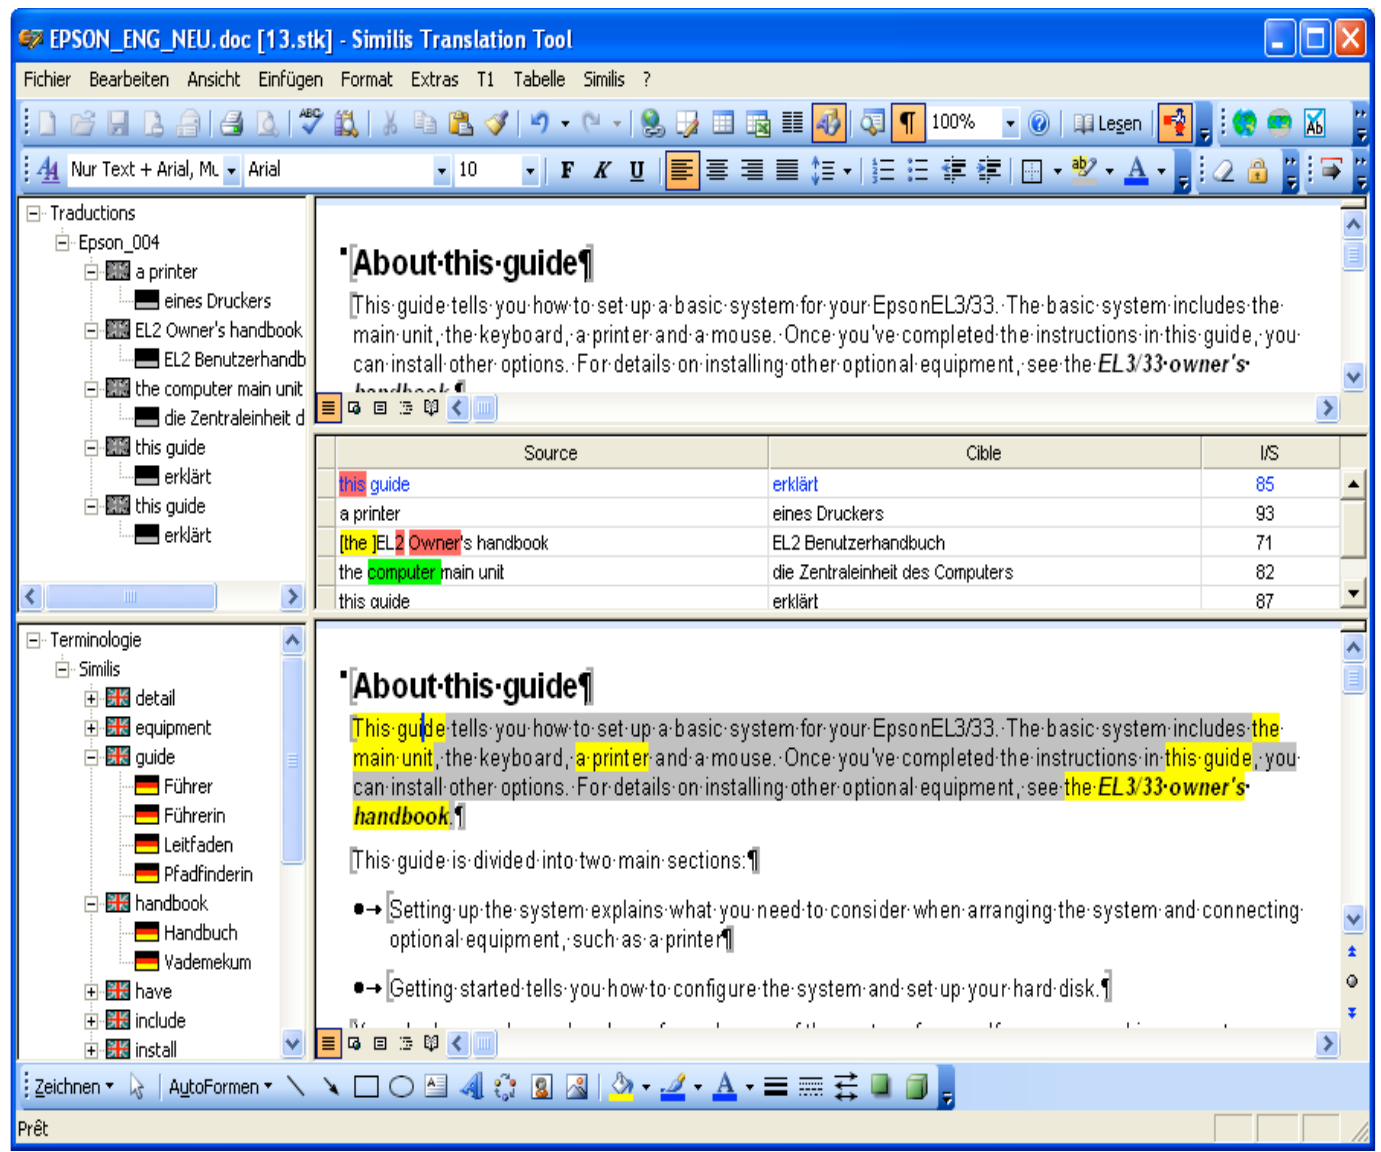
\includegraphics[width=\textwidth]{figures/ReinkeF11.png} 
\end{figure}

\begin{figure}
\caption{Subsegment alignment in Similis\label{fig:reinke:12}}
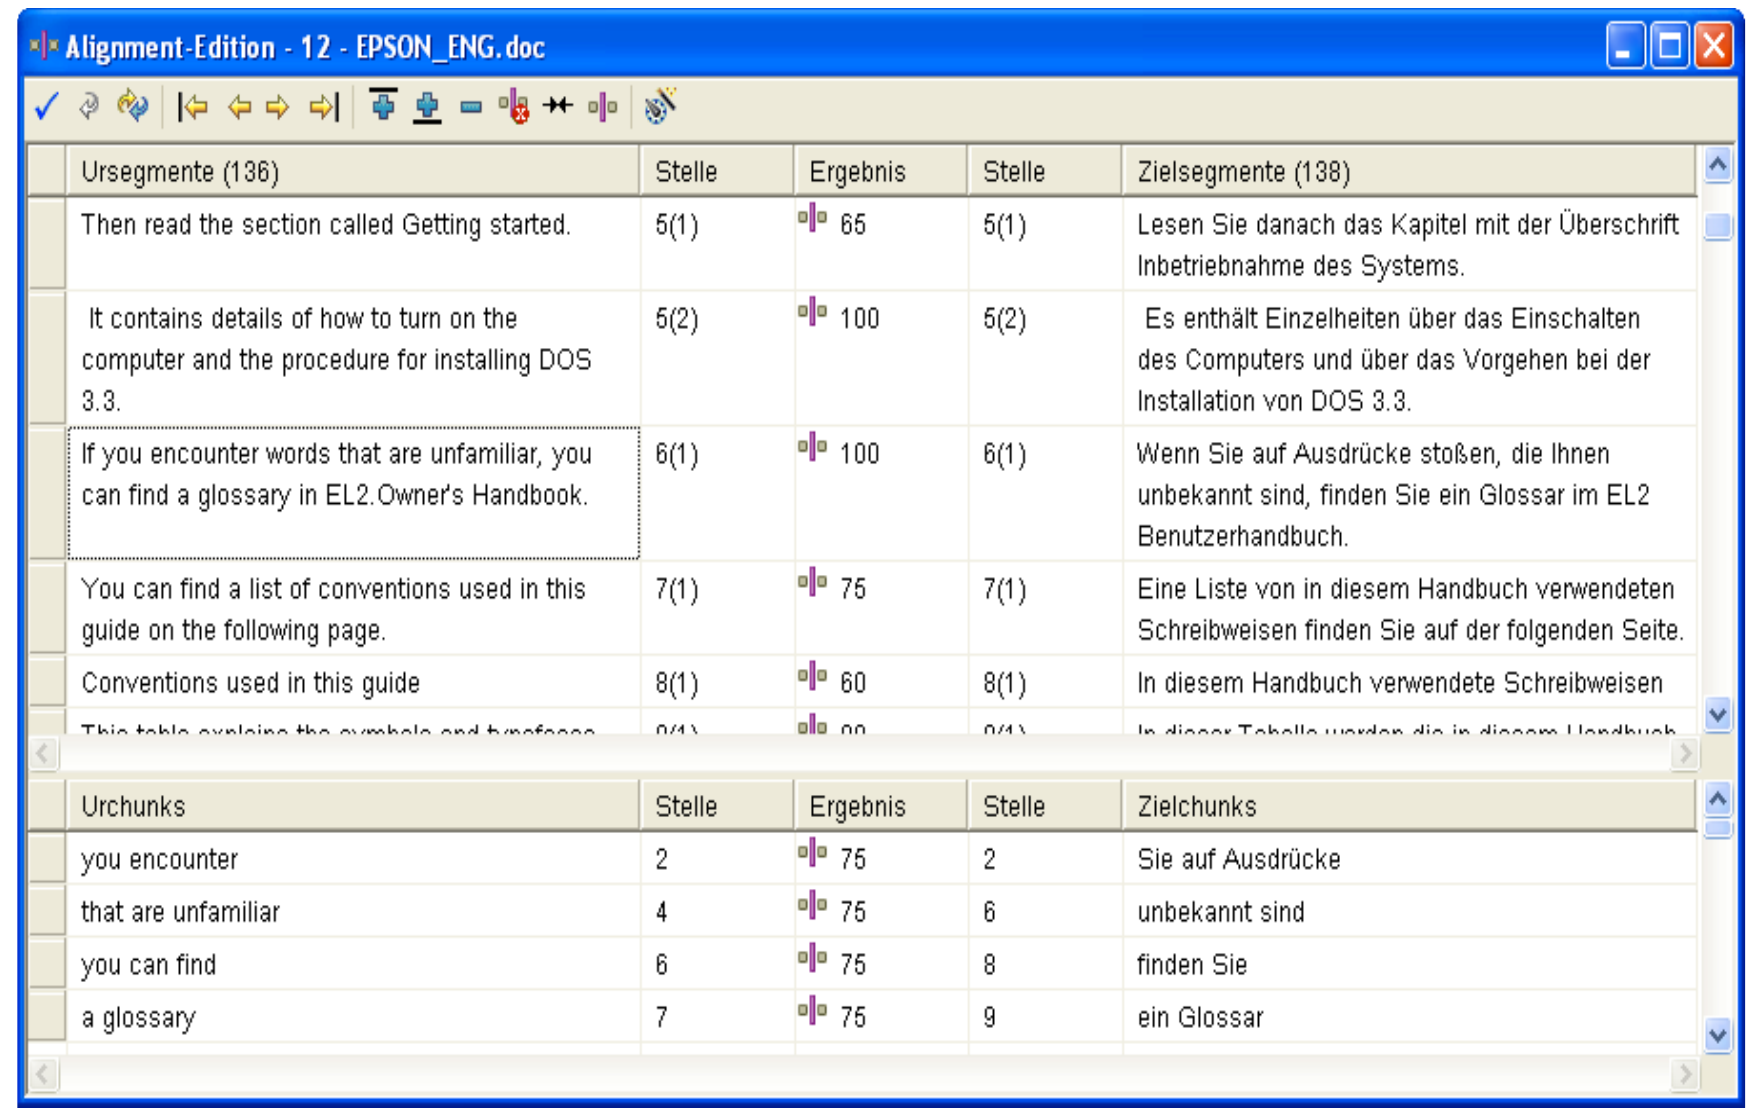
\includegraphics[width=\textwidth]{figures/ReinkeF12.png} 
\end{figure}

More recent research on enhancing retrieval in \textsc{tm} systems mainly seems to focus on improving the reusability of fuzzy matches by applying methods from \textsc{smt} (\citealt{Biçici2008}; \citealt{Zhechev2010}; \citealt{KoehnSenellart2010}). The aim is to identify those fragments that make the difference between a segment to be translated and a fuzzy match retrieved from a \textsc{tm} database and adjust their translations automatically using \textsc{smt} procedures. Ideally, for the human translator there would be no additional post-editing effort for these matches. However, one should have a careful ``empirical look'' at the question how this ``fusion'' of human translation and machine translation at segment level actually affects the post-editing of fuzzy matches and at what extent it really enhances the productivity of human translators as well as text quality.

\subsubsection{Integrating robust linguistic procedures into existing commercial systems}\label{sec:reinke:3.2.2}
 
Ways of integrating standard methods and procedures known from computational linguistics into commercial \textsc{tm} systems are currently analyzed at Cologne University of Applied Sciences in a research project supported by the German Federal Ministry of Education and Research (\textsc{bmbf}) \citep{AzzanoEtAl2011}. The focus of the project lies on enhancing the performance of commercial \textsc{tm} systems with respect to the retrieval of paraphrase patterns and subsegment fragments as well as on improving term recognition and validation with the help of robust procedures for morphosyntactic and sentence syntactic analysis. The goal is to develop interface models and prototypical interfaces between commercial \textsc{tm} systems and ``lingware'' using \textsc{sdl} Trados Studio 2009 and the morphosyntactic analysis tool \textsc{mpro} \citep{Maas2009} as a prototypical environment and German and English as prototypical languages to gain experiences for the development of further language modules and for applying the results to other \textsc{tm} systems.
 
At first, relevant similarity patterns were identified and classified using authentic multilingual technical documentation (user manuals and operating instructions from various areas). For this purpose, \textsc{tm} databases were created and compared with ``related'' texts (updates, texts on closely related items of communication, texts belonging to related text types and dealing with the same topic of communication). Currently the master \textsc{tm} database contains 51.000 segments. Both the segments from the \textsc{tm} databases and the texts ``related'' to the \textsc{tm} material were morphosyntactically annotated with \textsc{mpro}. To identify relevant similarity patterns the ``related'' texts were automatically matched with the \textsc{tm} databases using the pretranslate function. In many cases the resulting match values and the similarity judgments of human translators differed considerably. In a further step, the linguistic differences between the segments of the new, ``related'' texts and the matches from the \textsc{tm} were described and categorized in order to identify linguistic features that may help to enhance the retrieval performance of commercial \textsc{tm} systems.
 
To integrate morphosyntactical information into the commercial \textsc{tm} a stand-alone \textsc{sql} database was developed. This ``linguistic \textsc{tm}'' is built from the morpho-syntactically annotated segments of the commercial \textsc{tm} and -- apart from the tokens of the text surface -- mainly contains information obtained from lemmatization, compound analysis and word class recognition. The segments of the ``linguistic \textsc{tm}'' are linked to the ``originals'' in the commercial \textsc{tm} via unique \textsc{id}s. To accelerate the retrieval of relevant \textsc{tu}s from the \textsc{sql} database the data is stored in the form of suffix arrays \citep{Aluru2004}.
 
When looking up \textsc{tu}s in the ``linguistic \textsc{tm}'' during the translation process each SLSeg first need to be morphosyntactically analyzed and annotated. The actual retrieval process then consists of two steps. First, the tokens found in the SLSeg to be translated are compared with the tokens in the SLSeg\textsubscript{TMling} to determine whether one or more SLSeg\textsubscript{TMling} completely or partially contain SLSeg. A second query searches the ``linguistic \textsc{tm}'' for all SLSeg\textsubscript{TMling} with morphosyntactic patterns similar to those of the SL\textsubscript{Seg} to be translated. For all results of both queries the Longest Common Substrings (\textsc{lcs}) between SL\textsubscript{Seg} and SLSeg\textsubscript{TMling} are calculated using Generalized Suffix Arrays (\textsc{gsa}) \citep{Rieck2007}. In order to rank the results a formula is developed that combines the matches obtained from the two queries taking into consideration the number and the length of \textsc{lcs} as well as their position in SL\textsubscript{Seg} and SLSeg\textsubscript{TMling} \citep{Hawkins2009}.
 

\section{Conclusions and outlook}\label{sec:reinke:4}
 
This paper has given an overview of the state of the art in \textsc{tm} technology, explaining the major concepts and looking at recent trends in both commercial systems and research. As \textsc{tm} and \textsc{mt} ``have been developed very much in isolation'' because ``different communities played a role in each technology's development'' \citep{KoehnSenellart2010} and computational linguistics has long ignored the relevance of \textsc{tm} as a major language technology used in professional translation, there is still ample scope for further research as well as for closer collaboration between academia and the language translation industry.
 
An important field that could not be touched upon in this paper for reasons of space and time is empirical research on how \textsc{tm} and \textsc{mt} and the combination of both actually integrate into the translation workflow and how they influence the work of the translator. \citet[99]{Christensen2010}, identified three different areas of empirical \textsc{tm} research, namely ``technology-oriented'', ``workflow-oriented'' and ``translation-theoretical'', and conclude that  

\begin{quotation}
Empirically documented knowledge about the nature and applications of \textsc{tm} systems and translators' interaction with them is both scarce and fragmented. In particular, more research is needed on how translators interact with \textsc{tm} technology and on how it influences translators' cognitive processes. The translation profession itself will also welcome more knowledge about the translators' perspective on \textsc{tm} technology. \citep[99]{Christensen2010}
\end{quotation}

Research into these areas has only just begun and it is to be hoped that in the near future more funding will be made available in this direction, because language technology for a multilingual society must, like any technology, serve the needs of its users.

\sloppy
\printbibliography[heading=subbibliography,notkeyword=this]

\end{document} 


